\documentclass[aspectratio=43]{beamer}
\usepackage{ragged2e}
\usepackage{multirow}
\usepackage{alltt}

\usetheme{CSCS}


\newcommand{\SummerSchoolYear}{2016}
\newcommand{\SummerSchoolDate}{July 20 -- 21}
\newcommand{\SummerSchoolAuthor}{Maxime Martinasso}

\newcommand{\footlinetext}{Summer School \SummerSchoolYear{} -- MPI}

\author{\SummerSchoolAuthor, CSCS}
\title{Message Passing Interface (MPI)}
\subtitle{Summer School \SummerSchoolYear{}  -- Effective High Performance Computing}
\date{\SummerSchoolDate, \SummerSchoolYear}


% Select the image for the title page
\newcommand{\picturetitle}{cscs_images/image3.pdf}
%\newcommand{\picturetitle}{cscs_images/image5.pdf}
%\newcommand{\picturetitle}{cscs_images/image6.pdf}

\begin{document}

% TITLE SLIDE
\cscstitle

\begin{frame}{Previous course summary}
\begin{itemize}
\item Point-to-point communication, Blocking and non-blocking
\item Collective operations
\item Derived datatypes
\end{itemize}
\end{frame}

\begin{frame}{Course Objectives}
\begin{itemize}
\item The understanding of a topology and communicators
\item How to build and use a topology
\end{itemize}
\end{frame}

% TABLE OF CONTENT SLIDE
\cscstableofcontents[hideallsubsections]{General Course Structure}

\section{An introduction to MPI}
\section{Point-to-point communications}
\section{Collective communications}
\section{Datatypes}
\section{Topology}
\cscstableofcontents[currentsection]{General Course Structure}

% CHAPTER SLIDE
\cscschapter{Topology}

\subsection{Groups and communicator}

\begin{frame}[fragile]{Groups and communicator}
\begin{itemize}
\item A group is an ordered set of processes, each with a unique integer rank. In MPI, a group is represented within system memory as an object. It is accessible to the programmer only by a "handle". A group is always associated with a communicator object.
\item A communicator encompasses a group of processes that may communicate with each other. All MPI messages must specify a communicator. Like groups, communicators are accessible to the programmer only by "handles". The handle for the communicator that comprises all processes is \verb+MPI_COMM_WORLD+.
\end{itemize}
From the programmer's perspective, a group and a communicator are
one. The group routines are primarily used to specify which
processes should be used to construct a communicator.
\end{frame}

\begin{frame}[fragile]{Groups and communicator}
\begin{columns}
\begin{column}{0.5\paperwidth}
\textbf{Goals:}
\begin{itemize}
\item Allow you to organize tasks, based upon function, into task groups.
\item Enable Collective Communications operations across a subset of related tasks.
\item Provide basis for implementing user defined virtual topology.
\end{itemize}
\textbf{Remarks:}
Groups/communicators can be created and destroyed during program execution.
Processes may be in more than one group/communicator having a unique rank within each group/communicator.
\end{column}
\begin{column}{0.5\paperwidth}
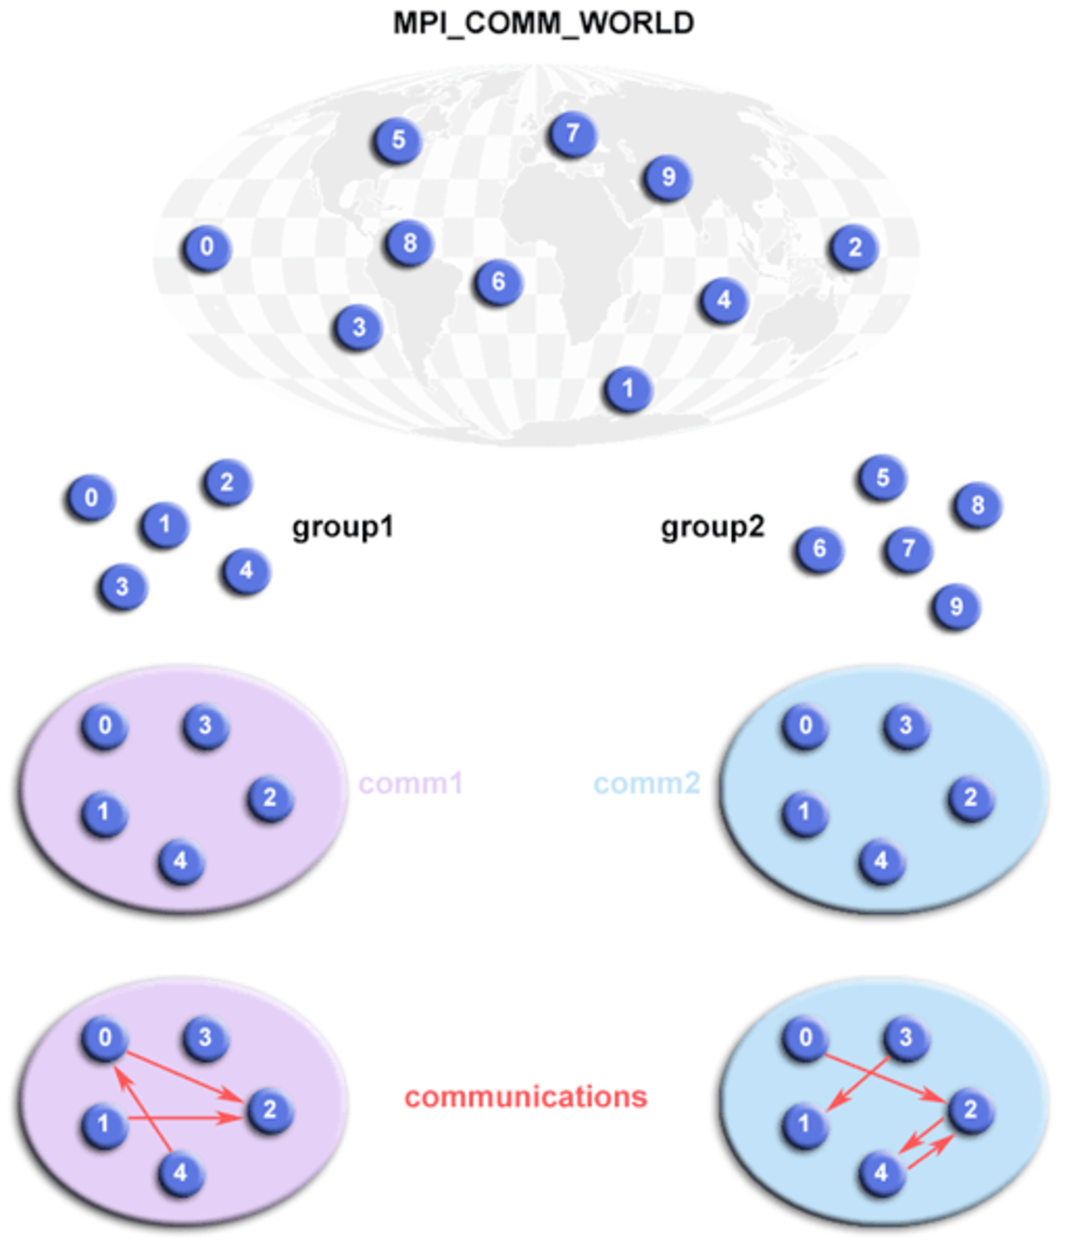
\includegraphics[scale=0.36]{05.MPI_Topo/world.pdf}
\end{column}
\end{columns}
\end{frame}


\begin{frame}[fragile]{Defining a new communicator: the simple approach}
\begin{Fortranlisting}[]{}
MPI_group MPI_GROUP_WORLD
MPI_group first_row_group
MPI_Comm first_row_comm
Integer row_size
Parameter(row_size=2)
Integer process_ranks(row_size)

Do i = 1, row_size
   process_ranks(i) = i-1
Enddo

Call MPI_COMM_GROUP(MPI_COMM_WORLD, MPI_GROUP_WORLD, ierr)

Call MPI_GROUP_INCL(MPI_GROUP_WORLD, row_size,
                    process_ranks, first_row_group, ierr)

Call MPI_COMM_CREATE(MPI_COMM_WORLD, first_row_group, first_row_comm, ierr)
\end{Fortranlisting}
\end{frame}

\begin{frame}[fragile]{Defining a new communicator: the smart approach}
\begin{Pseudolisting}[]{}
MPI_Comm_split(comm, color, key, comm_out)
\end{Pseudolisting}
\begin{black1block}{}
\begin{tabular}{rp{8cm}}
\textbf{color} & identifies the group\\
    \textbf{key} & specifies a member of the group (rank)\\
\end{tabular}
\end{black1block}
\begin{columns}
\begin{column}{0.2\paperwidth}
\begin{tabular}{|c|c|}
    \multicolumn{2}{c}{6 ranks} \\\hline
    P0 & P1 \\\hline
    P2 & P3 \\\hline
    P4 & P5 \\\hline
\end{tabular}
\end{column}
\begin{column}{0.2\paperwidth}
\begin{tabular}{|c|c|}
    \multicolumn{2}{c}{row\_comm} \\\hline
    \color{cscsred}P0 & \color{cscsred}P1 \\\hline
    \color{cscsgreen}P2 & \color{cscsgreen}P3 \\\hline
    \color{cscsblue}P4 & \color{cscsblue}P5 \\\hline
\end{tabular}
\end{column}
\begin{column}{0.19\paperwidth}
\begin{tabular}{|c|c|}
    \multicolumn{2}{c}{col\_comm} \\\hline
    \color{cscsred}P0 & \color{cscsblue}P1 \\\hline
    \color{cscsred}P2 & \color{cscsblue}P3 \\\hline
    \color{cscsred}P4 & \color{cscsblue}P5 \\\hline
\end{tabular}
\end{column}
\begin{column}{0.41\paperwidth}
\begin{tabular}{|c|c|c|c|c|c|c|}
    \multicolumn{7}{c}{} \\\hline
myRank & 0 & 1 & 2 & 3 & 4 & 5 \\\hline
iRow & 0 & 0 & 1 & 1 & 2 & 2 \\\hline
jCol & 0 & 1 & 0 & 1 & 0 & 1 \\\hline
\end{tabular}
\end{column}

\end{columns}
\begin{Fortranlisting}[]{}
! logical 2D topology with nrow=3 rows and mcol=2 columns
! 6 ranks, it is a collective operation
iRow = myRank/mcol       !! logical row number
jCol = mod(myRank, mcol) !! logical column number

Call MPI_COMM_SPLIT(MPI_COMM_WORLD, iRow, jCol, row_comm, ierr)
Call MPI_COMM_SPLIT(MPI_COMM_WORLD, jCol, iRow, col_comm, ierr)
\end{Fortranlisting}
\end{frame}


\subsection{Topology with MPI}
\begin{frame}[fragile]{Topology with MPI}
\begin{itemize}
\item A virtual topology describes the "connectivity" of MPI processes in a communicator.
\item The two main types of topology are Cartesian and Graph.
\item MPI topology are virtual - there may be no relation between the physical structure of the parallel machine and the process topology.
\item Virtual topology are built upon MPI communicators and groups.
\end{itemize}
\begin{blue1block}{Cartesian topology}
\begin{itemize}
\item Each process is “connected” to its neighbors in a virtual grid
\item Boundaries can be cyclic
\item Identified by (discrete) Cartesian coordinates $(i, j, k)$
\end{itemize}
\end{blue1block}
\begin{blue1block}{Graph topology}
\begin{itemize}
\item Graphs are used to describe communication patterns
\item The most general description of communication patterns
\end{itemize}
\end{blue1block}
\end{frame}

\subsection{Domain decomposition}
\begin{frame}[fragile]{Domain decomposition}
\textbf{Planar distribution}: data are distributed “linearly” between processors.
Default mapping when using \verb+MPI_COMM_WORLD+.\\
\visible<2>{Ghost cells are exchanged: processor N communicates with N-1 and N+1}
\includegraphics<1>[scale=0.5]{05.MPI_Topo/decomp1.pdf}
\includegraphics<2>[scale=0.5]{05.MPI_Topo/decomp1gc.pdf}
\end{frame}

\begin{frame}[fragile]{Domain decomposition}
\textbf{Cartesian distribution}: data are distributed “linearly” between processors.
\vspace{0.5cm}
\begin{columns}
\begin{column}{0.322\paperwidth}
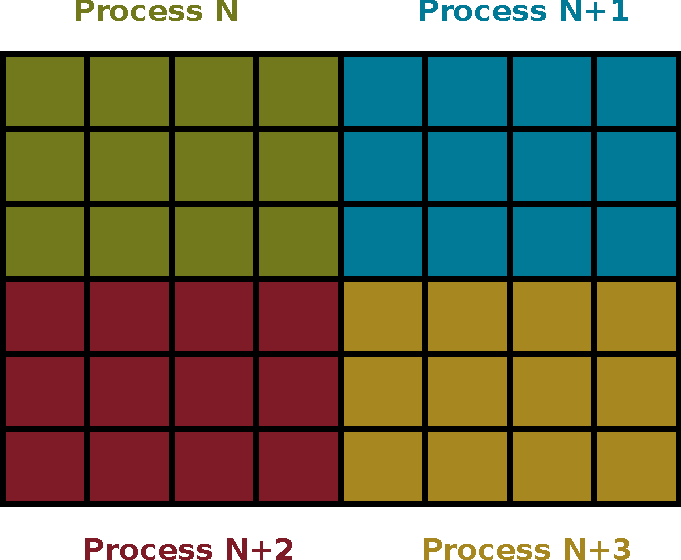
\includegraphics[scale=0.4]{05.MPI_Topo/decomp2.pdf}
\end{column}
\begin{column}{0.5\paperwidth}
This is in general a more effective way of distribute the domain, since:
\begin{itemize}
\item It is much more scalable
\item Communicated data volume can be smaller (especially when a large number of processors is used)
\item It can better map the geometry of the problem and of the algorithm
\end{itemize}
\end{column}
\end{columns}
\vspace{0.5cm}
However, it is more difficult to handle: who are my neighbors?
\end{frame}



\subsection{Cartesian topology}
\begin{frame}[fragile]{Cartesian topology}
\begin{Pseudolisting}[]{}
MPI_Cart_create(comm_old, ndims, dims, periods, reorder, 
                comm_cart)
\end{Pseudolisting}
\begin{black1block}{}
\begin{tabular}{rp{8cm}}
\textbf{comm\_old} & input communicator\\
\textbf{ndims} & number of dimensions of Cartesian grid\\
\textbf{dims} & specifies the number of processes in each dimension\\
\textbf{periods} & specifies whether the grid is periodic (true) or not (false) in each dimension\\
\textbf{reorder} & ranking may be reordered (true) or not (false)\\
\textbf{comm\_cart} & communicator with new Cartesian topology\\
\end{tabular}
\end{black1block}
\vspace{-0.3cm}
\begin{center}
Row-major numbering:\hspace{0.5cm}
\footnotesize
\begin{tabular}{|c|c|c|c|}
\hline
\color{cscsblue}0  & \color{cscsblue}1  & \color{cscsblue}2  & \color{cscsblue}3\\
    (0,0) & (0,1) & (0,2) & (0,3)\\\hline
\color{cscsblue}4  & \color{cscsblue}5  & \color{cscsblue}6  & \color{cscsblue}7\\
    (1,0) & (1,1) & (1,2) & (1,3)\\\hline
\color{cscsblue}8  & \color{cscsblue}9  & \color{cscsblue}10 & \color{cscsblue}11\\
    (2,0) & (2,1) & (2,2) & (2,3)\\\hline
\color{cscsblue}12 & \color{cscsblue}13 & \color{cscsblue}14 & \color{cscsblue}15\\
    (3,0) & (3,1) & (3,2) & (3,3)\\\hline
\end{tabular}
\end{center}
\end{frame}



\begin{frame}[fragile]{Cartesian topology example}
\footnotesize
\vspace{-1.3cm}
\begin{columns}
\begin{column}{0.55\paperwidth}
\begin{Fortranlisting}[]{}
INTEGER :: comm_cart
INTEGER :: ierr
INTEGER :: dims(3)
LOGICAL :: periods(3)

dims(1) = NprocX
dims(2) = NprocY
dims(3) = NprocZ
periods = .TRUE.

Call MPI_CART_CREATE(MPI_COMM_WORLD, 3, dims, periods, .TRUE., comm_cart, ierr)
\end{Fortranlisting}
\end{column}
\begin{column}{0.4\paperwidth}

\includegraphics[scale=0.36]{05.MPI_Topo/3dcube.pdf}
\end{column}
\end{columns}
\end{frame}

\begin{frame}[fragile]{Periods and reorder}

\textbf{Periods}: Define if the boundary of the grid are periodic or not.\\
\begin{center}
\begin{tabular}{cccccc}
    \multicolumn{6}{c}{periods = False} \\\hline
    \color{cscsred}-1 & $\leftarrow$\color{cscsblue}0 &\color{cscsblue}1 & \color{cscsblue}2 & {\color{cscsblue}3}$\rightarrow$ & \color{cscsred}-1\\\hline
    \multicolumn{6}{c}{periods = True} \\\hline
    \color{cscsred}3 & $\leftarrow$\color{cscsblue}0 & \color{cscsblue}1 & \color{cscsblue}2 & {\color{cscsblue}3}$\rightarrow$ & \color{cscsred}0\\\hline
\end{tabular}
\end{center}
Note: \lstinlinePseudo{MPI_PROC_NULL=-1}\\

\textbf{Reorder}: allows MPI processes reordered for efficiency, possibly so as to choose a good embedding of the virtual topology onto the physical machine.

\end{frame}

\begin{frame}[fragile]{Utility functions}
Create dimensions:
\begin{Pseudolisting}[]{}
MPI_Dims_create(nnodes, ndims, dims)
\end{Pseudolisting}

Retrieves Cartesian topology information associated with a communicator
\begin{Pseudolisting}[]{}
MPI_Cartdim_get(comm, ndims)
MPI_Cart_get(comm, ndims, dims, periods, coords)
\end{Pseudolisting}
Coordinates to rank:
\begin{Pseudolisting}[]{}
MPI_Cart_rank(comm, coords, rank)
\end{Pseudolisting}
Rank to coordinates:
\begin{Pseudolisting}[]{}
MPI_Cart_coords(comm, rank, maxdims, coords)
\end{Pseudolisting}
\end{frame}


\begin{frame}[fragile]{Finding neighbors: Shift}
\begin{columns}
\begin{column}{0.65\paperwidth}
\begin{Pseudolisting}[]{}
MPI_Cart_shift(comm, direction, disp, 
               rank1, rank2)
\end{Pseudolisting}
\begin{black1block}{}
\begin{tabular}{rp{8cm}}
\textbf{comm} & communicator with Cartesian structure\\
\textbf{direction} & coordinate dimension of shift\\
\textbf{disp} & displacement\\
\textbf{rank1} & rank of nearby process\\
\textbf{rank2} & rank of nearby process\\
\end{tabular}
\end{black1block}
\begin{Fortranlisting}[]{}
Call MPI_CART_SHIFT(comm_cart, 0, 1,
                    left, right, ierr)
Call MPI_CART_SHIFT(comm_cart, 1, 1,
                    front, rear, ierr)
Call MPI_CART_SHIFT(comm_cart, 2, 1,
                    down, up, ierr)
\end{Fortranlisting}

\end{column}
\begin{column}{0.3\paperwidth}
\vspace{4cm}
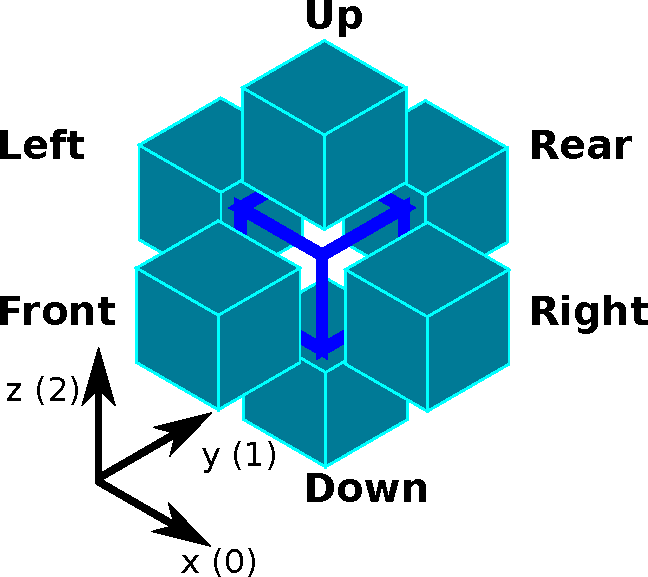
\includegraphics[scale=0.36]{05.MPI_Topo/shift.pdf}
\end{column}
\end{columns}

\end{frame}

\begin{frame}[fragile]{Sub-grids in Cartesian topology}
\begin{columns}
\begin{column}{0.5\paperwidth}
\begin{Pseudolisting}[]{}
MPI_Cart_sub(comm, remain_dims,
             newcomm)
\end{Pseudolisting}
\begin{black1block}{}
\begin{tabular}{rp{3cm}}
\textbf{comm} & communicator with Cartesian structure\\
\textbf{remain\_dims} & the ith entry of remain\_dims specifies whether the ith dimension is kept in the subgrid (true) or is dropped (false)\\
\textbf{newcom} & communicator containing the subgrid including the calling process\\
\end{tabular}
\end{black1block}
\end{column}
\begin{column}{0.49\paperwidth}
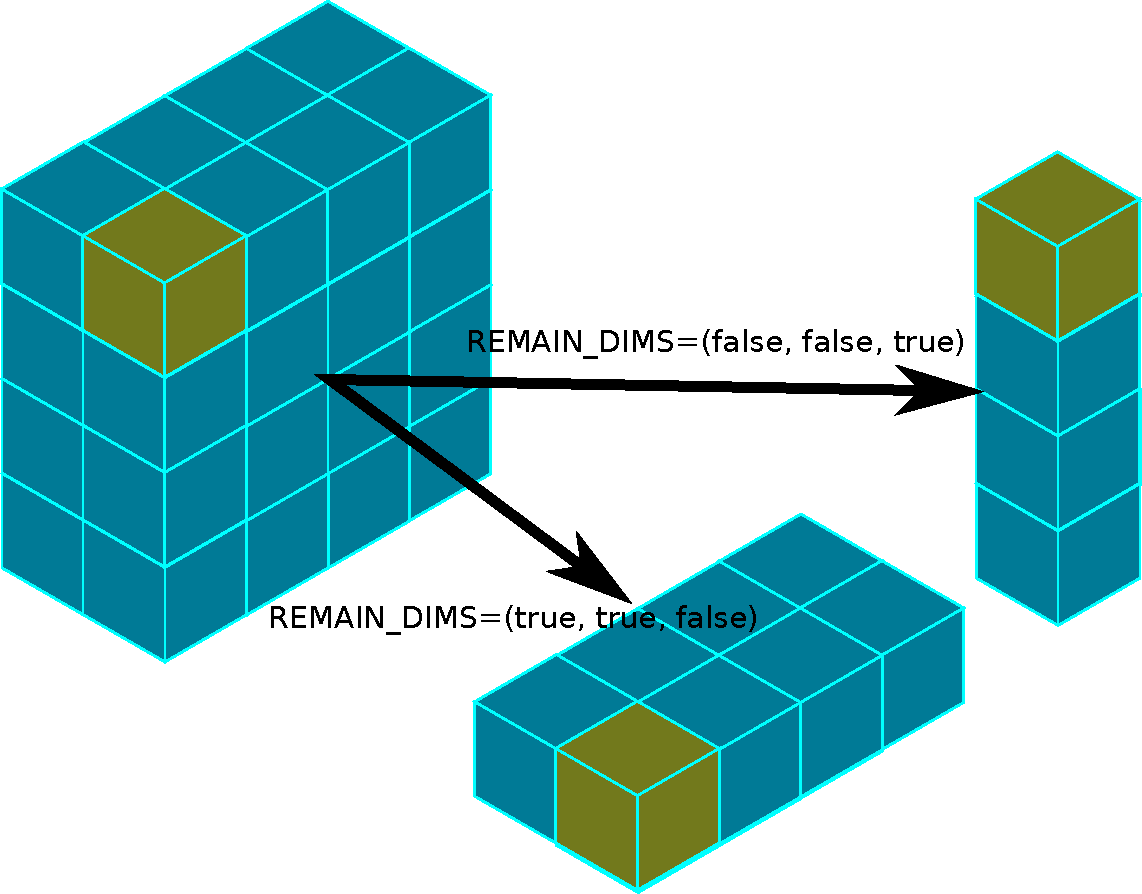
\includegraphics[scale=0.29]{05.MPI_Topo/subgrid.pdf}
\end{column}
\end{columns}
\end{frame}



\subsection{Graph topology}
\begin{frame}[fragile]{Graph topology}
\begin{Pseudolisting}[]{}
MPI_Graph_create(comm_old, nnodes, index, edges, reorder,
                 comm_graph)
\end{Pseudolisting}
\begin{black1block}{}
\begin{tabular}{rp{8cm}}
\textbf{comm\_old} & input communicator\\
\textbf{nnodes} & number of nodes in graph\\
\textbf{index} & array of integers describing node degrees\\
\textbf{edges} & array of integers describing graph edges\\
\textbf{reorder} & ranking may be reordered (true) or not (false)\\
\textbf{comm\_graph} & communicator with graph topology added\\
\end{tabular}
\end{black1block}
\begin{columns}
\begin{column}{0.3\paperwidth}
\begin{tabular}{|c|c|}\hline
    Process & Neighbors\\\hline
    0 & 1,3\\\hline
    1 & 0\\\hline
    2 & 3\\\hline
    3 & 0,2\\\hline
\end{tabular}
\end{column}

\begin{column}{0.3\paperwidth}
\begin{black1block}{}
nnodes = 4\\
index = 2, 3, 4, 6\\
edges = 1, 3, 0, 3, 0, 2\\
\end{black1block}
\end{column}

    \begin{column}{0.2\paperwidth}
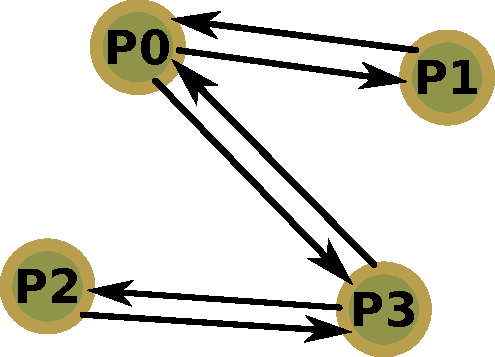
\includegraphics[scale=0.36]{05.MPI_Topo/graph.pdf}
    \end{column}
\end{columns}

\end{frame}


\begin{frame}[fragile]{Other functions}
\begin{itemize}
    \item Manage communicators:\\\hspace{1cm}\lstinlinePseudo{MPI_Comm_compare, MPI_Comm_dup} \ldots
    \item Manipulate groups:\\\hspace{1cm}\lstinlinePseudo{MPI_Group_union, MPI_Group_intersection} \ldots
        \item Cartesian topology, map a process:\\\hspace{1cm}\lstinlinePseudo{MPI_Cart_map}
        \item Graph topology:\\\hspace{1cm}\lstinlinePseudo{MPI_Graph_map, MPI_Graph_get} \ldots
\end{itemize}
\end{frame}


\begin{frame}{Practicals}
    \begin{brown2block}{Exercise: 05.MPI\_Topo}
    \begin{enumerate}
        \item Create a 1-dimension topology - a ring
        \item Ghost cell exchanges using a topology
    \end{enumerate}
    \end{brown2block}
\end{frame}




% THANK YOU SLIDE
\cscsthankyou{Thank you for your attention.}

\end{document}
